\documentclass[uplatex,dvipdfmx,a4paper,11pt]{jsarticle}

\usepackage{docmute}


% 数式
\usepackage{amsmath,amsthm,amssymb}
\usepackage{bm}
% 画像
\usepackage{graphicx}

\usepackage{multirow}
\usepackage{wrapfig}
\usepackage{ascmac}
\usepackage{xcolor}


\usepackage{makeidx}
\makeindex

\graphicspath{{../../_Figures//}{../../_Figures/Rheology/}}

\usepackage{qrcode}
\setlength\lineskiplimit{0pt}
\setlength\normallineskiplimit{0pt}

\usepackage{qexam}

\usepackage{titlesec}
\titleformat*{\section}{\Large\bfseries}
\titleformat*{\subsection}{\large\bfseries}
\titleformat*{\subsubsection}{\normalsize\bfseries}
\titleformat*{\paragraph}{\normalsize\bfseries}

% ページ設定
% \pagestyle{empty}
% 高さの設定
\setlength{\textheight}{\paperheight}   % ひとまず紙面を本文領域に
\setlength{\topmargin}{-5.4truemm}      % 上の余白を20mm(=1inch-5.4mm)に
\addtolength{\topmargin}{-\headheight}  % 
\addtolength{\topmargin}{-\headsep}     % ヘッダの分だけ本文領域を移動させる
\addtolength{\textheight}{-40truemm}    % 下の余白も20mmに%% 幅の設定
\setlength{\textwidth}{\paperwidth}     % ひとまず紙面を本文領域に
\setlength{\oddsidemargin}{-5.4truemm}  % 左の余白を20mm(=1inch-5.4mm)に
\setlength{\evensidemargin}{-5.4truemm} % 
\addtolength{\textwidth}{-40truemm}     % 右の余白も20mmに
% 図と本文との間
%\abovecaptionskip=-5pt
%\belowcaptionskip=-5pt
%
% 全体の行間調整
% \renewcommand{\baselinestretch}{1.0} 
% 図と表
%\renewcommand{\figurename}{Fig.}
%\renewcommand{\tablename}{Tab.}
%

% \makeatletter 
% \def\section{\@startsection {section}{1}{\z@}{1.5 ex plus 2ex minus -.2ex}{0.5 ex plus .2ex}{\large\bf}}
% \def\subsection{\@startsection{subsection}{2}{\z@}{0.2\Cvs \@plus.5\Cdp \@minus.2\Cdp}{0.1\Cvs \@plus.3\Cdp}{\reset@font\normalsize\bfseries}}
% \makeatother 

\usepackage[dvipdfmx,%
 bookmarks=true,%
 bookmarksnumbered=true,%
 colorlinks=false,%
 setpagesize=false,%
 pdftitle={数式に頼らない直感的理解による材料設計のためのレオロジー⼊⾨},%
 pdfauthor={佐々木裕},%
 pdfsubject={},%
 pdfkeywords={レオロジー; 材料設計; }]{hyperref}
\usepackage{pxjahyper}

\usepackage{plext}

\usepackage{niceframe} 
\usepackage{framed}
\newenvironment{longartdeco}{%
  \def\FrameCommand{\fboxsep=\FrameSep \artdecoframe}%
  \MakeFramed {\FrameRestore}}%
 {\endMakeFramed}
 
\usepackage{siunitx}

\newcommand{\rmd}{\mathrm{d}}

\usepackage[inline]{showlabels}

\begin{document}

\question{演習問題 1}
内容を振り返るために、以下に示した文章例の中から適切な記述のものを複数選んでください。
\begin{qlist}
	\qitem 「固体と液体の応答」についての、正しい言葉はどれでしょうか?
		\begin{qlist2}
			\qitem 固体のモデルでは応力は加えたひずみに反比例します。
			\qitem 液体のモデルでは応力はひずみ速度に比例します。
			\qitem 固体でも液体でも、力の釣り合いを考えれば十分です。
			\qitem 液体では時間の因子が重要になります。
			\qitem 実際の物質では、粘性と弾性を併せ持ったものが多く存在します。
		\end{qlist2}
		\vspace{3mm}

	\qitem マックスウェルモデルについての、正しい言葉はどれでしょうか?
		\begin{qlist2}
			\qitem 粘弾性体の力学的な応答は、マックスウェルモデルで表すことができます。
			\qitem マックスウェルモデルは、バネとダッシュポットが並列に横に並んだモデルです。
			\qitem マックスウェルモデルでは、応力はバネとダッシュポットで異なる値となります。
			\qitem マックスウェルモデルでは、ひずみがバネとダッシュポットに分割されます。
			\qitem バネが応力の弾性的挙動を、ダッシュポットが流動の粘性的挙動を表します。
		\end{qlist2}
		\vspace{3mm}

	\qitem 応力緩和についての、正しい言葉はどれでしょうか?
		\begin{qlist2}
			\qitem 応力緩和とは、物質に力を加えて保持し、変形ひずみが減少する過程を測定します。
			\qitem マックスウェルモデルは、応力緩和を記述できます。
			\qitem 応力緩和とは、粒子が居心地を改善していく過程と考えることができます。
			\qitem 粒子が居心地を改善する過程が、バネの弾性的な応答に対応します。
			\qitem 粒子が居心地を改善する過程に伴い、局所的な応力が消失します。
		\end{qlist2}
		\vspace{3mm}

	\qitem 緩和時間についての、正しい言葉はどれでしょうか?
		\begin{qlist2}
			\qitem マックスウェルの方程式は、応力緩和を記述できる微分方程式です。
			\qitem 応力緩和現象では、時間が経過すると応力が指数関数的に増加します。
			\qitem 緩和時間とは、応力が初期値の半分になる時間です。
			\qitem 緩和時間とは粘度と弾性率の比であり、どちらが支配的であるかを表します。
			\qitem 緩和時間は弾性率に反比例するので、弾性的であれば短くなります。
		\end{qlist2}
		\vspace{3mm}

	\qitem 一般化マックスウェルモデルについての、正しい言葉はどれでしょうか?
		\begin{qlist2}
			\qitem 実際の物質は、複雑な緩和挙動を示します。
			\qitem それぞれの緩和時間ごとに、一つ以上のマックスウェルモデルを対応させることができます。
			\qitem 一般化マックスウェルモデルとは、複数のマックスウェルモデルを縦に直列に連結したものです。
			\qitem 一般化マックスウェルモデルを用いても単純な緩和挙動しか記述できません。
			\qitem 粘弾性的に見た固体とは、長時間放置しても緩和しない応力成分が残存するものと考えることができます。
		\end{qlist2}

\end{qlist}

\question{演習問題 2}
内容を振り返るために、テキストで用いた言葉を使って簡単な穴埋めを行ってください。
\begin{qlist}
	\qitem 「粘性と弾性についての再確認」について、\qbox{(a)}から\qbox{(j)}までのカッコを埋めてください。
		\vspace{5mm}
		\begin{qlist2}
			\qitem 「固体と液体の応答」について
				\begin{center}
					\begin{tabular}{|c||c|} \hline
						固体のモデル & 液体のモデル \\ \hline \hline
						応力は\qbox{}に比例 & 応力は\qbox{}に比例\\ \hline
						% $\text{応力} = \text{弾性率} \times \text{ひずみ}$	& $\text{応力} = \text{粘度} \times \text{ひずみ速度}$ \\ \hline
						比例定数が\qbox{}& 比例定数が\qbox{}\\ \hline
						% 弾性率の単位は、[Pa] & 粘度の単位は、[Pa$\cdot$s]\\ \hline
						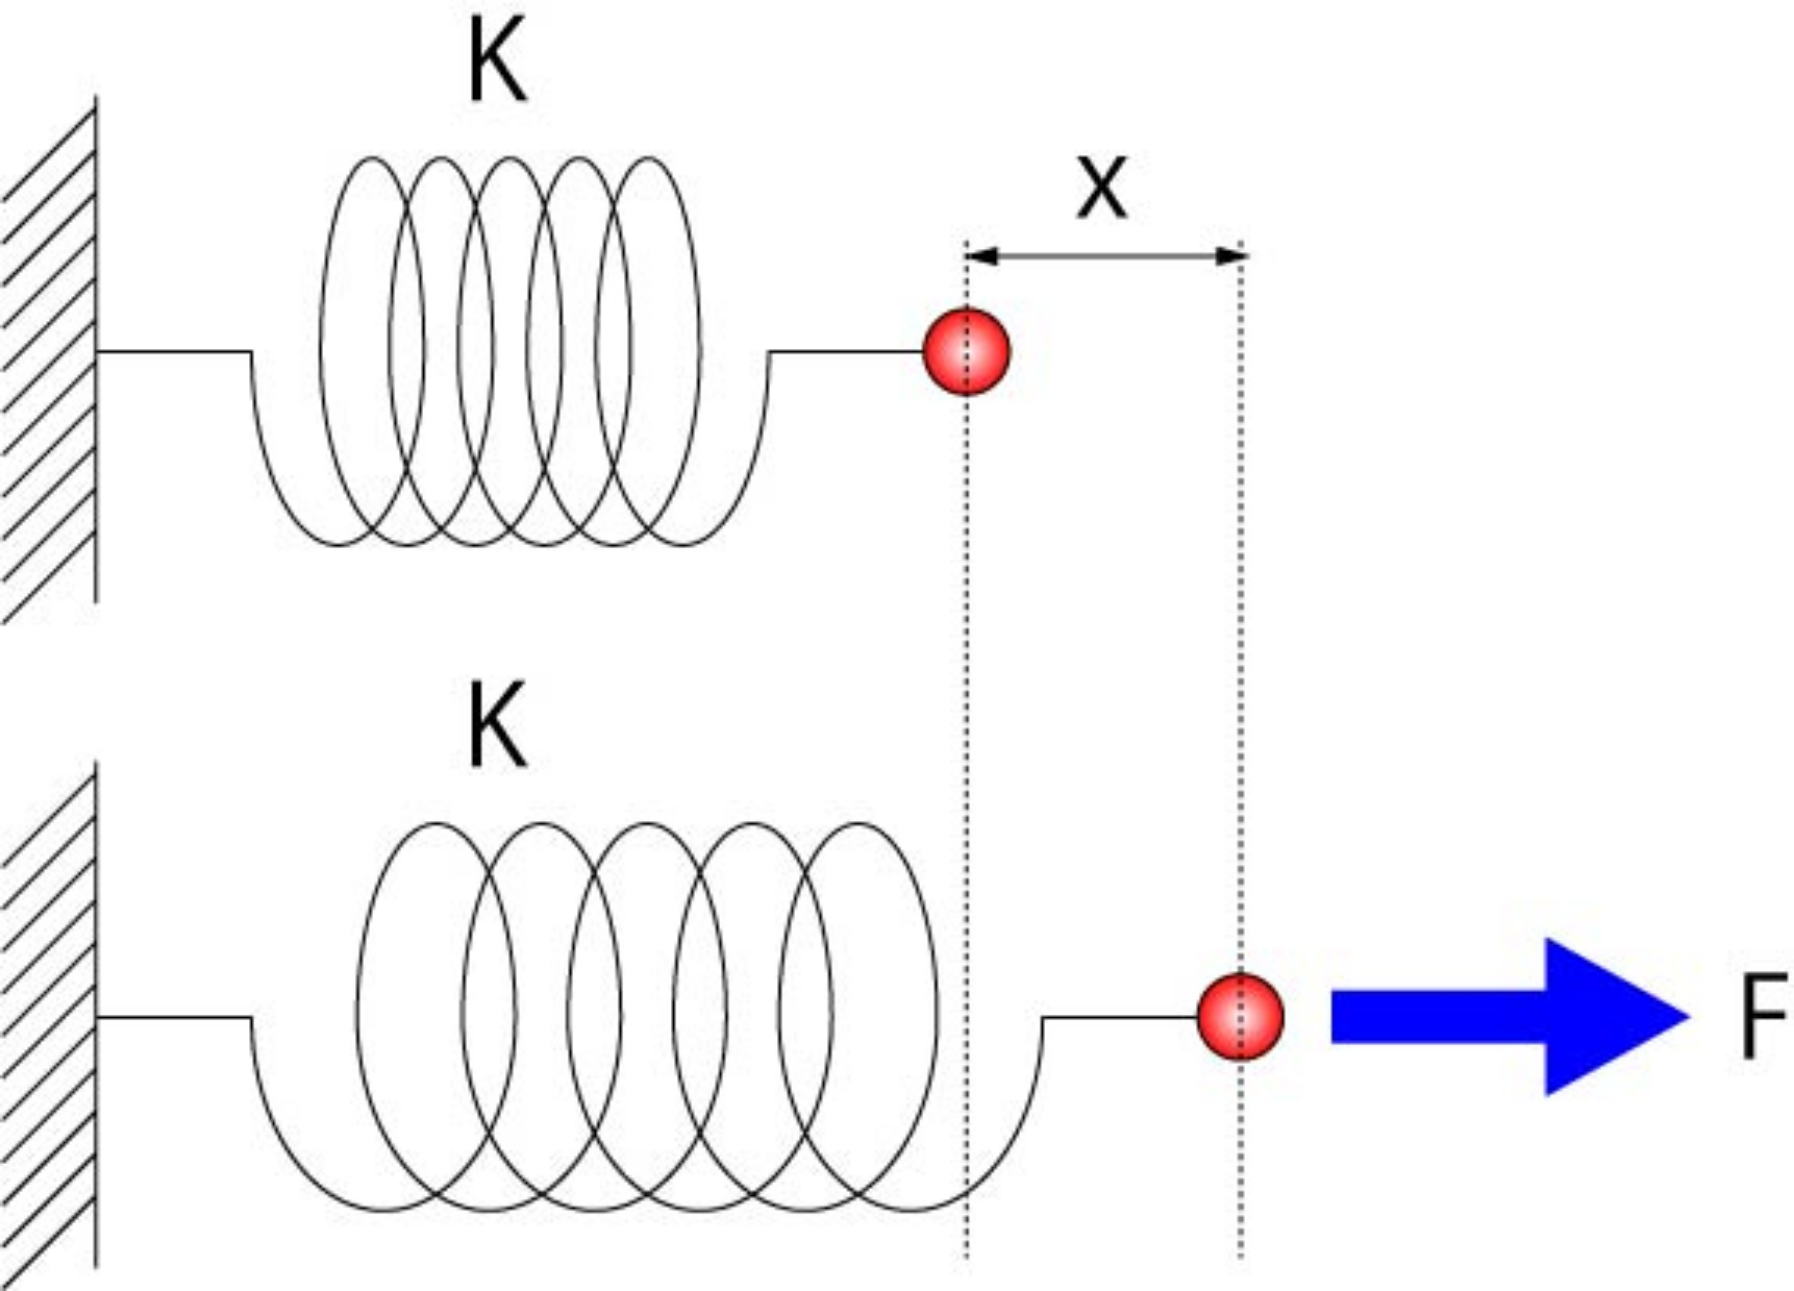
\includegraphics[width= 0.4\textwidth]{spring.png} & 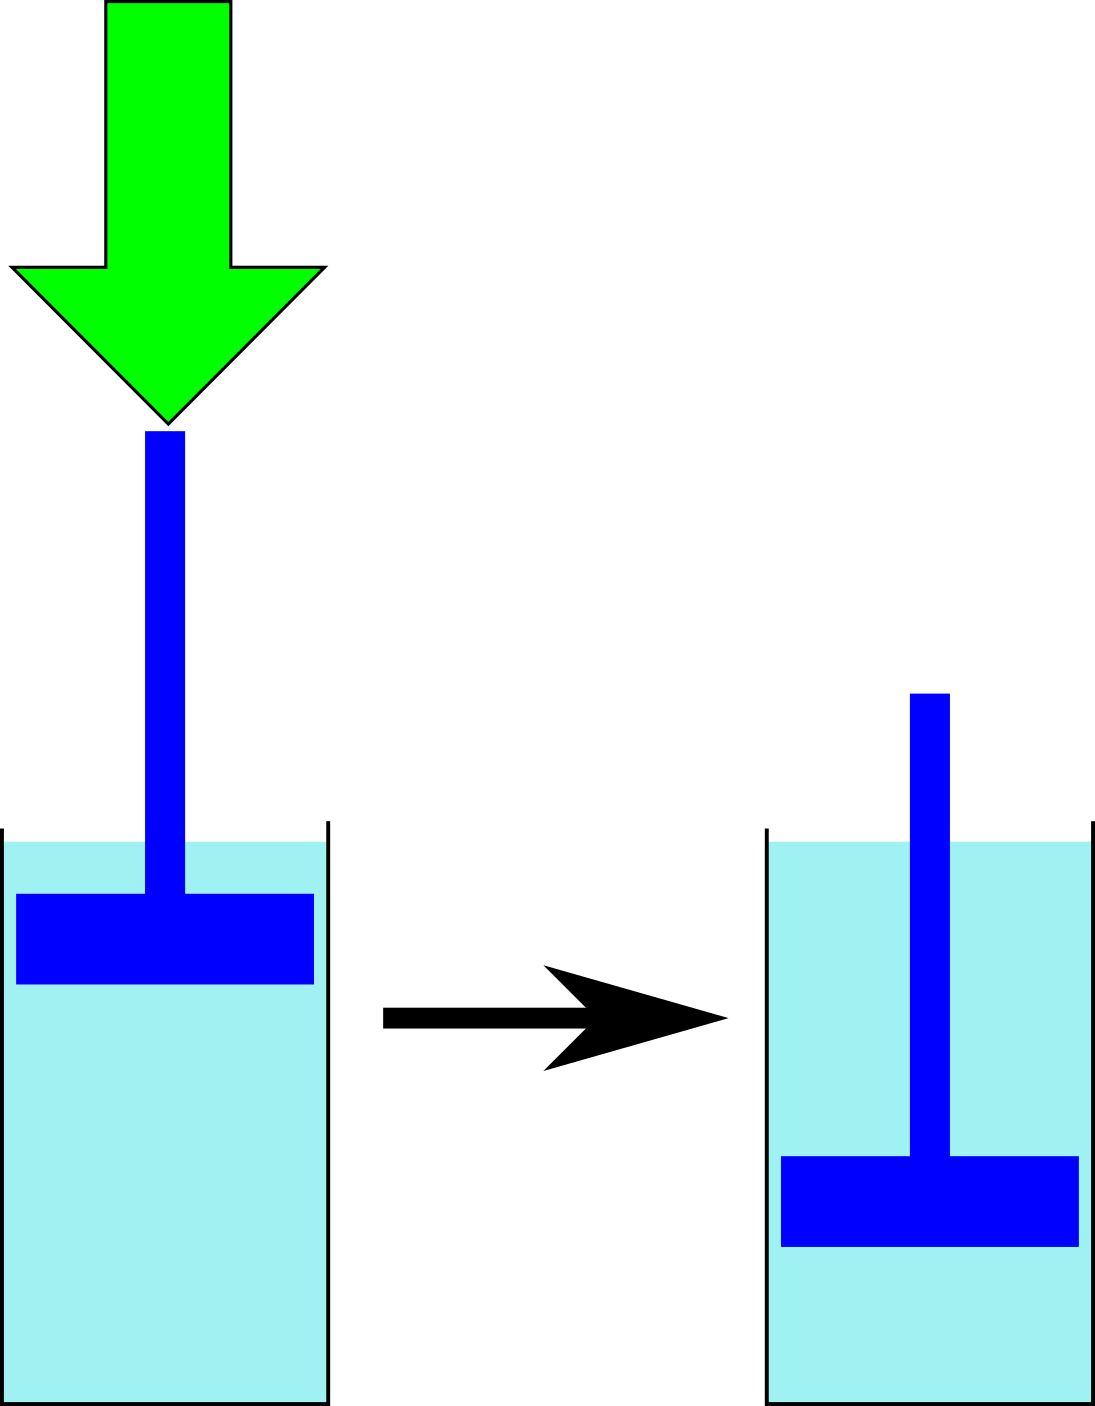
\includegraphics[width=.4\textwidth]{dashpot.png} \\ \hline
						力の\qbox{}&  \qbox{}の因子が重要 \\ \hline
					\end{tabular}
				\end{center}


			\vspace{5mm}
			\qitem 複雑な実事象について
				\begin{center}
					\begin{minipage}{0.4\textwidth}
						\begin{itemize}
							\item ビンガム氏の分類によれば、弾性変形という\qbox{}な応答を示すグループと、
							流れるという\qbox{}な応答を示すグループに分けられています。
							\item 結局、我々の身の回りにある物質の力学的な応答は、固体と液体と言うように単純に二分されるわけでもなく、
							\qbox{}と\qbox{}を併せ持ったものが多く存在することがわかります。
						\end{itemize}
					\end{minipage}
					\begin{minipage}{0.46\textwidth}
						\begin{center}
						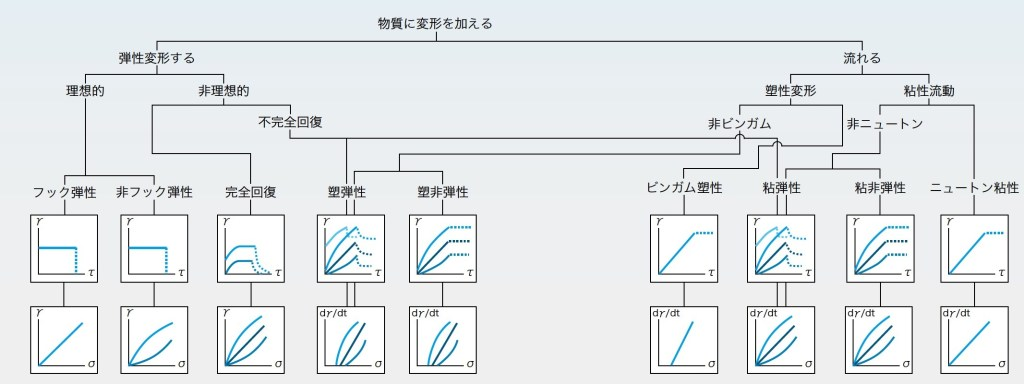
\includegraphics[width=\textwidth]{reoroji.jpeg}
						\end{center}
					\end{minipage}
				\end{center}

		\end{qlist2}

		\begin{itembox}[l]{選択肢}
			\begin{center}
				\begin{tabular}{lllll}
					1. 粘性	&2. 粘度	&3. ひずみ	&4. 固体的	&5. 弾性率\\
					6. 弾性	&7. ひずみ速度		&8. 釣り合い	&9. 液体的 &10. 時間
				\end{tabular}
			\end{center}
		\end{itembox}
\end{qlist}

\begin{qlist}
	\qitem 「粘弾性のモデル化」について、\qbox{(k)}から\qbox{(s)}までのカッコを埋めてください。
		\vspace{5mm}
		\begin{qlist2}
			\qitem マックスウェルモデルとは
			\begin{center}
				\begin{minipage}{0.4\textwidth}
					\begin{itembox}[l]{マックスウェルモデルの数式}
						\begin{itemize}
							\item \qbox{}モデル
							\begin{align*}
								\sigma_s(t) = E \varepsilon_s(t)
							\end{align*}
							\item \qbox{}モデル
							\begin{align*}
								\sigma_d(t) = \eta \dfrac{\mathrm{d}}{\mathrm{d}t}\varepsilon_d(t)
							\end{align*}
							\item \qbox{}に連結だから、
							\begin{itemize}
								\item 応力は\qbox{}
							\item ひずみは\qbox{}
							\end{itemize}
						\end{itemize}	
					\end{itembox}
				\end{minipage}
				\begin{minipage}{0.45\textwidth}
					\begin{center}
					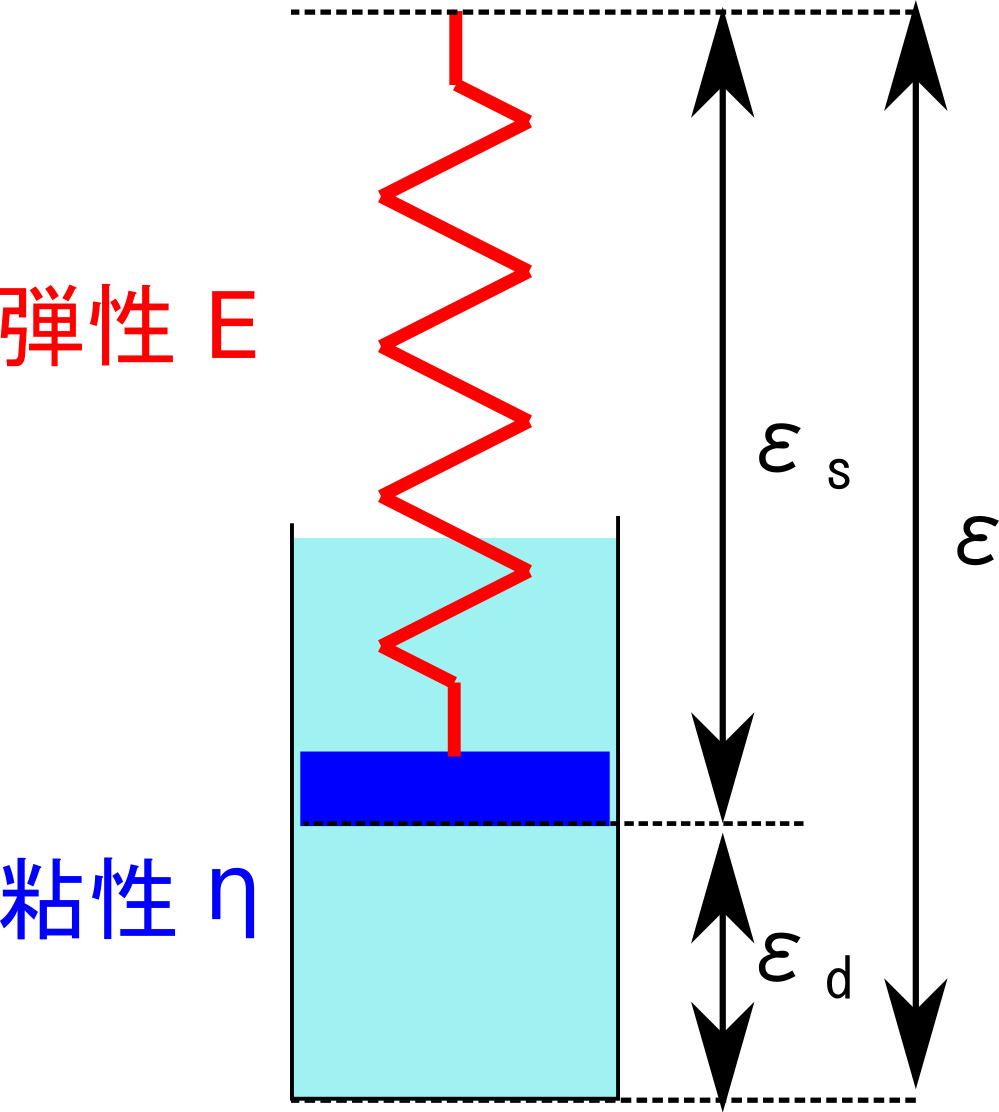
\includegraphics[width=.6\textwidth]{Maxwell_model.png}
					\end{center}
					\begin{align*}
						\begin{cases}
							\sigma = \sigma_s = \sigma_d \\
							\varepsilon = \varepsilon_s + \varepsilon_d
						\end{cases}
					\end{align*}
				\end{minipage}
			\end{center}

			\vspace{5mm}
			\qitem 一般化マックスウェルモデルでの緩和
			\begin{center}
				\begin{minipage}{0.86\textwidth}
					\begin{itembox}[l]{一般化マックスウェルモデルの緩和挙動}
						\begin{itemize}
							\item 個々のマックスウェルモデルの\qbox{}の\qbox{}の形で記述され、
							\item 仮に緩和強度が同一とすると、右図のように単純な和となり、
							\item \qbox{}に従って、緩和時間の\qbox{}ものから順次緩和していく。
						\end{itemize}
					\end{itembox}
				\end{minipage}
				\begin{minipage}{0.43\textwidth}
					\begin{center}
						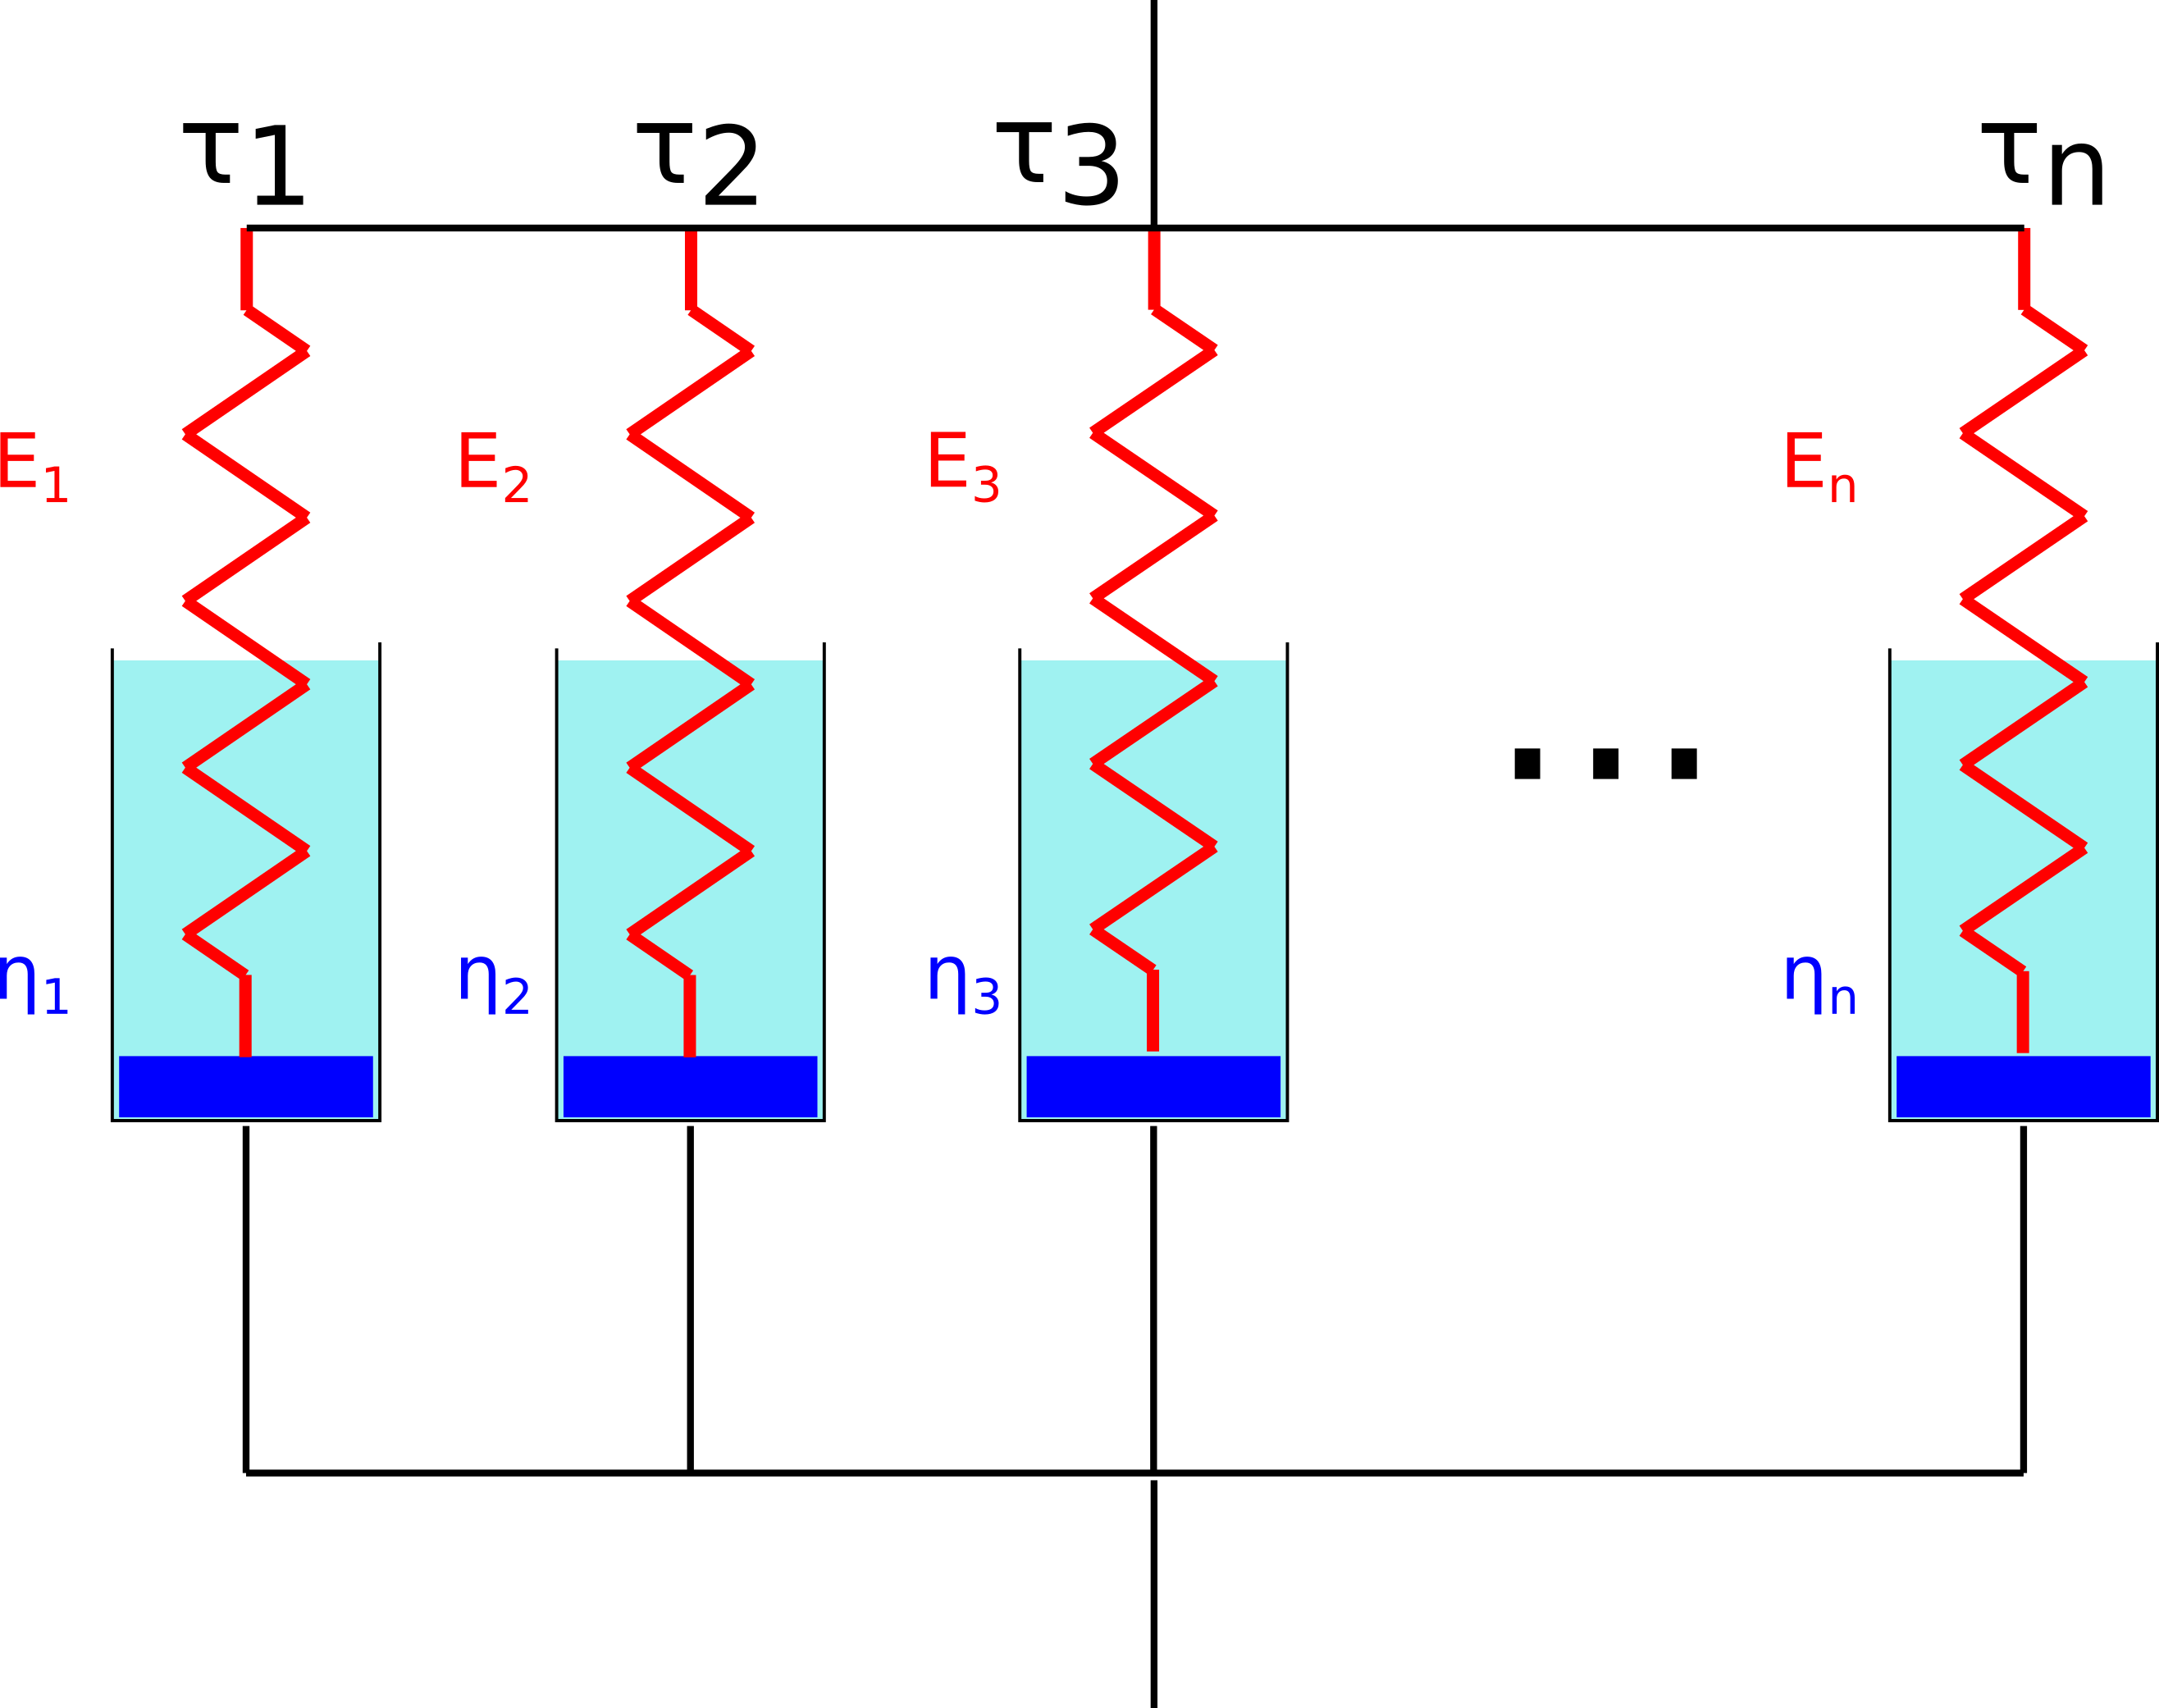
\includegraphics[width=\textwidth]{Maxwell_multi_1.png}
					\end{center}
				\end{minipage}
				\begin{minipage}{0.43\textwidth}
					\begin{center}
						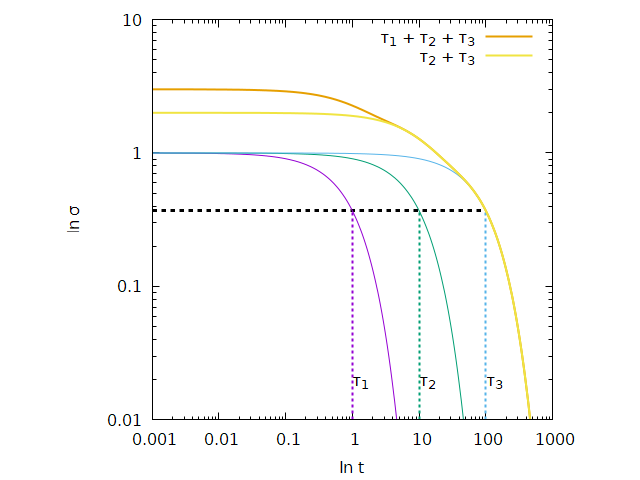
\includegraphics[width=\textwidth]{relux_8.png}
					\end{center}
				\end{minipage}
			\end{center}
				
		\end{qlist2}

		\begin{itembox}[l]{選択肢}
			\begin{center}
				\begin{tabular}{lllll}
					1. 緩和挙動	&2. 弾性	&3. 時間	&4. 短い	&5. 共通\\
					6. それぞれの和	&7. 粘性		&8. 和	&9. 直列
				\end{tabular}
			\end{center}
		\end{itembox}
\end{qlist}


\question{演習問題 3}
説明文中の言葉を使って数行程度の簡単な記述で構いませんので、以下の自由記述問題を考えてみてください。
\begin{qlist}
\qitem この章では、レオロジーの主たる対象である粘性と弾性を併せ持った粘弾性性質について、マックスウェルモデルという弾性を表すバネと粘性を表すダッシュポッ
トを直列に連結したモデルを用いて、変形時に物質中で生じた応力が緩和するというイメージの説明を行いました。

文中の言葉をそのまま使って結構ですから、ご自分なりの「粘弾性体が緩和するとはどういう現象なのか」ということを書いてみてください。
\end{qlist}


\clearpage


\end{document}